\documentclass[portuguese,11pt,a4paper,titlepage]{article}

\usepackage{graphicx}
\usepackage{fancyhdr}
\usepackage[portuguese]{babel}
\usepackage{blindtext}
\usepackage{listings}
\usepackage[T1]{fontenc}
\usepackage[margin=2.5cm]{geometry}
\usepackage[final]{pdfpages}
\usepackage{siunitx}
\usepackage[framed, numbered]{matlab-prettifier}
\usepackage{wrapfig}
\usepackage{subcaption}
\usepackage{hyperref}

\hypersetup{
    colorlinks,
    citecolor=black,
    filecolor=black,
    linkcolor=black,
    urlcolor=black
}

\setlength{\headheight}{14.2pt}
\fancypagestyle{fancy}{
	\fancyhf{}
	\fancyhead[C]{A02 -- word\_ladder}
	\fancyfoot[R]{
		\textsf{\thepage}
	}
	\fancyfoot[L]{
		\textsf{AED -- 2022/2023}
	}
	\fancyfoot[C]{
\includegraphics[height=.6cm]{ua.pdf}}
	\renewcommand{\headrulewidth}{0pt}
}
\pagestyle{fancy}

\definecolor{mygreen}{rgb}{0,0.6,0}
\definecolor{mygray}{rgb}{0.5,0.5,0.5}
\definecolor{mymauve}{rgb}{0.58,0,0.82}

\lstdefinestyle{c_without_comments}
{
	style=c_with_comments,
	morecomment  = [l][\@gobble]{//},
	morecomment  = [is]{/*}{*/},
}

\lstset{ 
	backgroundcolor=\color{white},   % choose the background color; you must add \usepackage{color} or \usepackage{xcolor}; should come as last argument
	basicstyle=\small\ttfamily,      % the size of the fonts that are used for the code
	breakatwhitespace=false,         % sets if automatic breaks should only happen at whitespace
	breaklines=true,                 % sets automatic line breaking
	captionpos=b,                    % sets the caption-position to bottom
	commentstyle=\color{mygreen},    % comment style
	extendedchars=true,              % lets you use non-ASCII characters; for 8-bits encodings only, does not work with UTF-8
	frameround=tttt,
	frame=single,	                 % adds a frame around the code
	keepspaces=true,                 % keeps spaces in text, useful for keeping indentation of code (possibly needs columns=flexible)
	keywordstyle=\color{blue},       % keyword style
	language=C,                      % the language of the code
	morekeywords={*,\ldots},         % if you want to add more keywords to the set
	numbers=none,                    % where to put the line-numbers; possible values are (none, left, right)
	rulecolor=\color{black},         % if not set, the frame-color may be changed on line-breaks within not-black text (e.g. comments (green here))
	showspaces=false,                % show spaces everywhere adding particular underscores; it overrides 'showstringspaces'
	showstringspaces=false,          % underline spaces within strings only
	showtabs=false,                  % show tabs within strings adding particular underscores
	stringstyle=\color{mymauve},     % string literal style
	tabsize=2,                       % sets default tabsize to 2 spaces
}

\newcommand{\foreign}[1]{\textit{#1}}
\newcommand{\srcdir}{..}
\newcommand{\hashtablegrowdir}{\srcdir/hash\_table\_grow-test}

\title{ \normalsize Licenciatura em Engenharia Informática\vskip 1.5em
		\Huge Algoritmos e Estruturas de Dados\vskip .7em
		\bfseries word\_ladder\vskip 1.5em
		
\includegraphics{ua.pdf}
}
\author{
	João Catarino\\NMec: 93096\and Rúben Garrido\\NMec: 107927\and Nuno Vieira\\NMec: 107283
}
\date{\today}
\addto\captionsportuguese{\renewcommand*\contentsname{Índice}}

\begin{document}
\maketitle

\tableofcontents
\pagebreak

\section{Introdução}
Texto aqui

\pagebreak
\section{Análise do incremento da \foreign{hash table}}
Por padrão, o tamanho inicial da \foreign{hash table} é 1000. No entanto, quando o número de entradas começa a ser significativo, começam a surgir colisões, o que implica uma perca da complexidade computacional \begin{math}O(1)\end{math}. Para evitar este problema, quando o rácio entre o tamanho da \foreign{hash table} e o número de colisões é superior a 5, o tamanho da \foreign{hash table} é incrementado, através da função \lstinline|hash_table_grow|, que recebe como argumento a referida \foreign{hash table}.

Contudo, a escolha do fator de incremento deve ser ponderada, já que, se for muito pequeno, o número de colisões diminui pouco, e se for muito grande, existe demasiada memória alocada não utilizada, o que leva a um desperdício de recursos. É esta escolha que pretendemos analisar.

\subsection{Explicação do código}
Foi desenvolvida uma nova função \lstinline|hash_table_grow|, num programa à parte, onde, após ser verificada a condição de incremento (rácio entre o tamanho da \foreign{hash table} e o número de colisões), é percorrido um ciclo \lstinline|for|, onde são testados vários valores de \lstinline|j| (fator de incremento).

\lstinputlisting[firstline=17, lastline=22]{\hashtablegrowdir/latex-hash\_table\_grow-test.c}

Dentro deste ciclo, e após definir inicializar algumas variáveis (p.e., a nova \foreign{hash table} temporária), surgem dois novos ciclos \lstinline|for|.

No primeiro \lstinline|for|, é percorrida a \foreign{hash table} inicial, onde, para cada \lstinline|node|, é calculado o novo índice, através do resto da divisão entre o valor retornado da função \lstinline|crc32| e o tamanho da \foreign{hash table}. Após este cálculo, é verificada a existência de colisões no índice calculado anteriormente, e, caso existam, é incrementado o valor de \lstinline|colnum|. Por fim, é associado o nó atual à nova \foreign{hash table}, na localização definida pelo índice.

\lstinputlisting[firstline=28, lastline=40]{\hashtablegrowdir/latex-hash\_table\_grow-test.c}

No segundo \lstinline|for|, é percorrida a nova \foreign{hash table}, onde é verificado o número de entradas livres desta. Caso \lstinline|test_new_table[k]| seja nulo, significa que a posição \lstinline|k| da \foreign{hash table} está livre, e, portanto, é incrementado o valor de \lstinline|free_entries|.

\lstinputlisting[firstline=41, lastline=45]{\hashtablegrowdir/latex-hash\_table\_grow-test.c}

Por fim, é impressa uma linha com os dados obtidos, nomeadamente o fator de incremento \lstinline|j|, o novo tamanho da \foreign{hash table} \lstinline|test_new_size|, a memória total ocupada \lstinline|test_new_size * sizeof(hash_table_node_t *)|, a memória ocupada por entradas livres \lstinline|free_entries * sizeof(hash_table_node_t *)| e o número de colisões \lstinline|colnum|.

\lstinputlisting[firstline=46, lastline=46]{\hashtablegrowdir/latex-hash\_table\_grow-test.c}

\subsection{Gráficos obtidos}
Através do MATLAB, foi possível obter um conjunto de gráficos, que relacionam colisões com memória livre e memória total. O script, disponível na secção \ref{MATLABcode}, obtém os dados através de um ficheiro de texto, que contém a tabela imprimida pelo programa de teste.

Os gráficos em questão incidem sobre o primeiro incremento, onde o tamanho atual da \foreign{hash table} é 1000.

\begin{figure}[h]
	\begin{subfigure}{0.47\textwidth}
		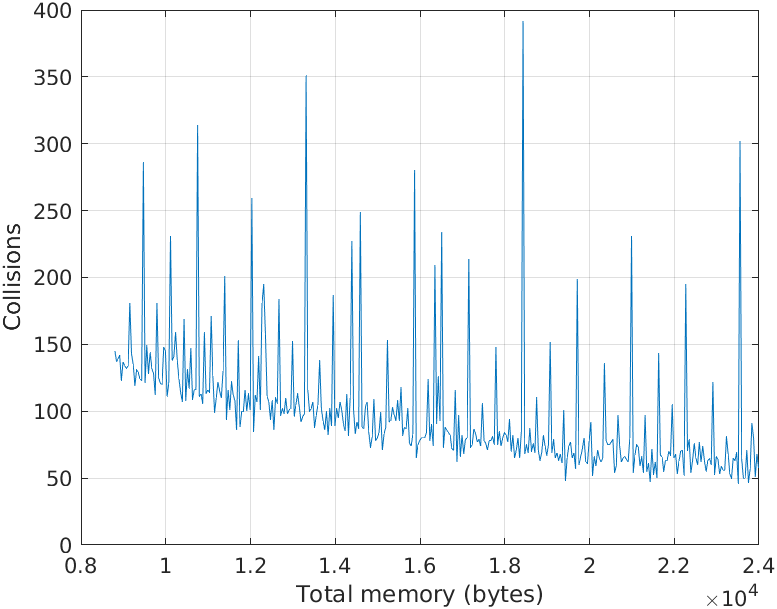
\includegraphics[width=\linewidth]{\hashtablegrowdir/plots/figure1.png} 
		\caption{Número de colisões em função da memória total.}
		\label{fig:htg_col_mem_total}
	\end{subfigure}
	\hspace{0.049\textwidth}
	\begin{subfigure}{0.47\textwidth}
		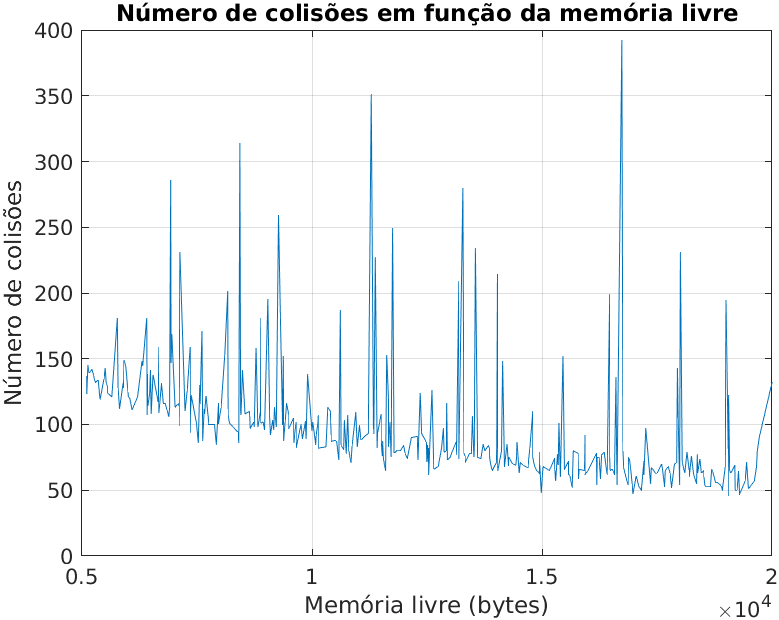
\includegraphics[width=0.96\linewidth]{\hashtablegrowdir/plots/figure2.png}
		\caption{Número de colisões em função da memória livre.}
		\label{fig:htg_col_mem_free}
	\end{subfigure}
	
	\caption{Número de colisões em função da memória.}
	\label{fig:htg_col_mem}
\end{figure}

\begin{figure}[h]
	\begin{subfigure}{0.47\textwidth}
		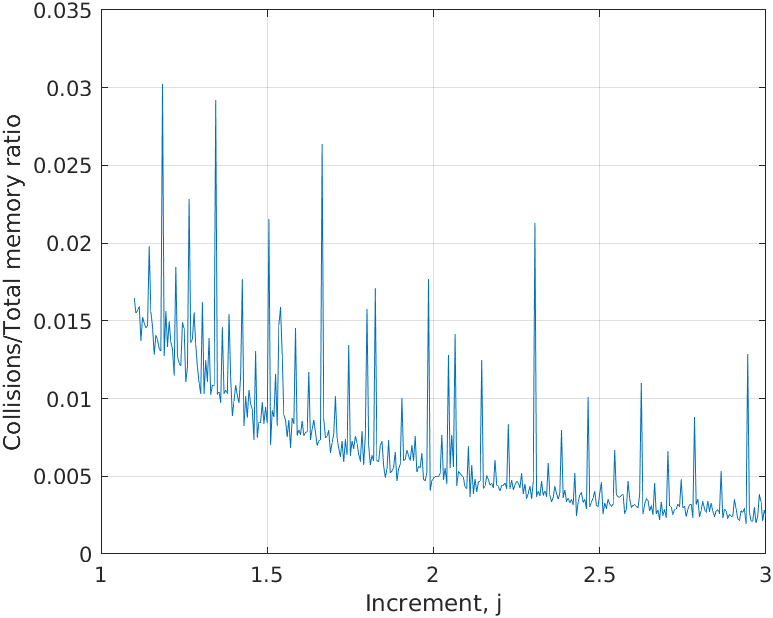
\includegraphics[width=0.96\linewidth]{\hashtablegrowdir/plots/figure3.png} 
		\caption{Rácio colisões/memória total.}
		\label{fig:htg_ratio_inc_total}
	\end{subfigure}
	\hspace{0.049\textwidth}
	\begin{subfigure}{0.47\textwidth}
		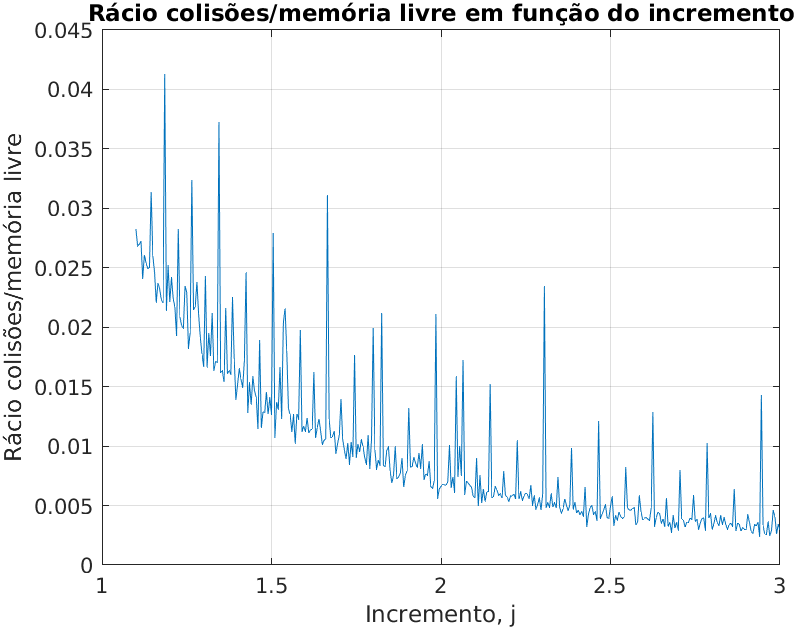
\includegraphics[width=\linewidth]{\hashtablegrowdir/plots/figure4.png}
		\caption{Rácio colisões/memória livre.}
		\label{fig:htg_ratio_inc_free}
	\end{subfigure}
	
	\caption{Rácio colisões/memória em função do incremento.}
	\label{fig:htg_ratio_inc}
\end{figure}

\begin{figure}[h]
	\centering
	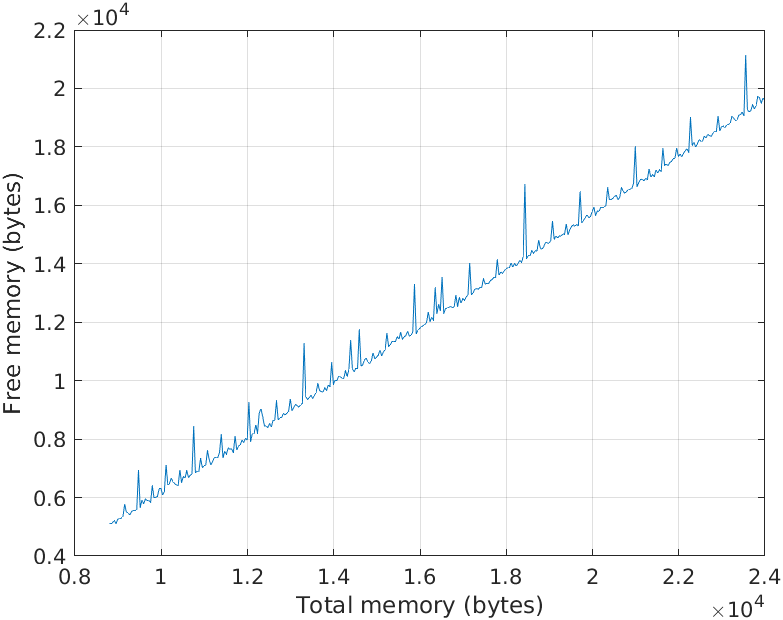
\includegraphics[width=0.47\linewidth]{\hashtablegrowdir/plots/figure5.png}
	\caption{Memória livre em função da memória total.}
	\label{fig:htg_free_total}
\end{figure}

\subsection{Análise dos resultados}
Em todos os gráficos, é possível observar irregularidades, associadas a uma maior ou menor quantidade de colisões. Isto deve-se ao facto de a \foreign{hash function} não ser perfeita e portanto, consoante o valor de \lstinline|j|, o índice associado a cada \lstinline|node| ser diferente, o que leva a colisões.

No entanto, é possível observar que, em geral, o número de colisões diminui com o aumento de memória (ou seja, com incrementos maiores), tal como seria esperado. A relação entre o número de colisões e a memória livre segue a mesma tendência. Em ambos os gráficos, verifica-se uma tendência aproximadamente linear.

Quanto aos rácios colisões/memória em função do incremento, observa-se em ambos os gráficos uma curva descendente, do tipo \begin{math}a \times x^b\end{math}, com \begin{math}-2 < b < -1\end{math}. Por este motivo, verifica-se uma diferença mais acentuada no eixo das ordenadas para incrementos menores do que para incrementos maiores. Assim, considera-se que o melhor incremento é o que apresenta um valor de \begin{math}b\end{math} mais próximo de 2, já que, a partir desse valor, o rácio tende a ser mais constante. Por outro lado, a similariedade entre rácios explica-se através do facto de a relação entre a memória livre e a memória total ser aproximadamente linear, com um declive próximo de 1 (ver figura \ref{fig:htg_free_total}).

No que diz respeito à relação entre a memória livre e a memória total (ambas em \foreign{bytes}), apesar das irregularidades, é possível efetuar uma regressão linear, onde se obtém a equação \begin{math}y=0.9583x-3357\end{math}.

Assim, uma vez que os gráficos não são completamente conclusivos quanto ao melhor fator de incremento, escolhemos utilizar o valor 2, já que este constitui um equilíbrio entre o número de colisões e a memória utilizada.

\pagebreak
\section{Código}
\subsection{Função hash\_table\_grow que testa o melhor incremento}
\lstinputlisting[firstline=4]{\hashtablegrowdir/latex-hash\_table\_grow-test.c}
\pagebreak
\subsection{Script MATLAB que gera os gráficos para análise da hash\_table\_grow} \label{MATLABcode}
\lstinputlisting[style=Matlab-editor, numbers=none, basicstyle=\small\ttfamily, firstline=5]{\hashtablegrowdir/script.m}
\end{document}